\documentclass[problem]{mcs}

\begin{pcomments}
  \pcomment{CP_simulating_fair_coin}
  \pcomment{from: S09.cp12r}
\end{pcomments}

\pkeywords{
  probability
}

%%%%%%%%%%%%%%%%%%%%%%%%%%%%%%%%%%%%%%%%%%%%%%%%%%%%%%%%%%%%%%%%%%%%%
% Problem starts here
%%%%%%%%%%%%%%%%%%%%%%%%%%%%%%%%%%%%%%%%%%%%%%%%%%%%%%%%%%%%%%%%%%%%%

% F09, S09

\begin{problem}
{\bf [Simulating a fair coin]}
Suppose you need a fair coin to decide which door to choose
in the 6.042 Monty Hall game.  After making everyone in your
group empty their pockets, all you managed to turn up is some crumpled
bubble gum wrappers, a few used tissues, and
one penny.  However, the penny was
from Prof. Meyer's pocket, so it is {\bf not} 
safe to assume that it is a fair coin.

How can we use a coin of unknown bias to get the same
effect as a fair coin of bias $1/2$? 
Draw the tree diagram for your solution, but since it is infinite,
draw only enough to see a pattern.

Suggestion:
A neat trick allows you to sum all the outcome probabilities
that cause you to  say "Heads":
Let $s$ be the sum of all "Heads" outcome probabilities in the whole
tree.  Notice that {\em you can write the sum of all the "Heads"
outcome probabilities in certain subtrees as a function of $s$}.  Use this
observation to write an equation in $s$ and then solve.

\begin{solution}
Flip Prof. Meyer's coin twice; if you see HT output Heads,
if you see TH output Tails, and if you
see HH or TT start over.

In the tree diagram in Figure~\ref{f-c}, the small triangles represent
subtrees that are themselves complete copies of the whole tree.

\begin{figure}[htbp]
\centerline{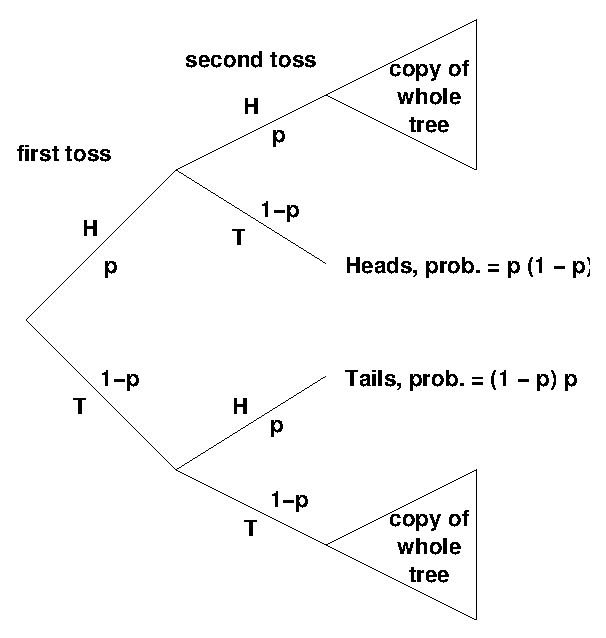
\includegraphics[width=0.40\textwidth]{figures/fair-coin}}
\caption{Simulating a Fair Coin.}
\label{f-c}
\end{figure}

Let $s$ equal the sum of all "Heads" probabilities in the whole tree.
There are two extra edges with probability $p$ on the path to each
outcome in the top subtree.  Therefore, the sum of "Heads" 
probabilities in the upper tree is $p^2 s$.  Similarly, the sum of
"Heads" probabilities in the lower subtree is $(1-p)^2 s$.  This gives
the equation:
\[
s = p^2 s + (1-p)^2 s + p (1-p)
\]

The solution to this equation is $s = 1/2$, for all $p$ between 0 and
1.
\end{solution}

\end{problem}


%%%%%%%%%%%%%%%%%%%%%%%%%%%%%%%%%%%%%%%%%%%%%%%%%%%%%%%%%%%%%%%%%%%%%
% Problem ends here
%%%%%%%%%%%%%%%%%%%%%%%%%%%%%%%%%%%%%%%%%%%%%%%%%%%%%%%%%%%%%%%%%%%%%

\endinput
